\documentclass{article}
\usepackage{amsmath}
\usepackage{amssymb}
\usepackage{indentfirst}
\usepackage{graphicx}
\usepackage{color}
\usepackage{fancyhdr}
\usepackage{epstopdf}
\usepackage{indentfirst}
\usepackage{geometry}
\geometry{left=2.5cm,right=2.5cm,top=2.5cm,bottom=2.5cm}

\title{14.03 Problem Set 4}
\author{Yijun Jiang}
%\email{yjjiang@mit.edu}
\date{\today}

\pagestyle{fancy}
\lhead{Yijun Jiang}
\rhead{14.03 Problem Set 4}

\begin{document}
\maketitle

\section{International Trade}
\subsection{Part 1}
Since $X=L_X$ and $Y=5\sqrt{L_Y}$, we have $L_X=X$ and $L_y=Y^2/25$. Therefore, the Finnish PPF is
\begin{equation*}
X+\frac{1}{25}Y^2=300
\end{equation*}

This PPF is plotted in Fig.\ref{PPF}.
\begin{figure}[!htbp]
\centering
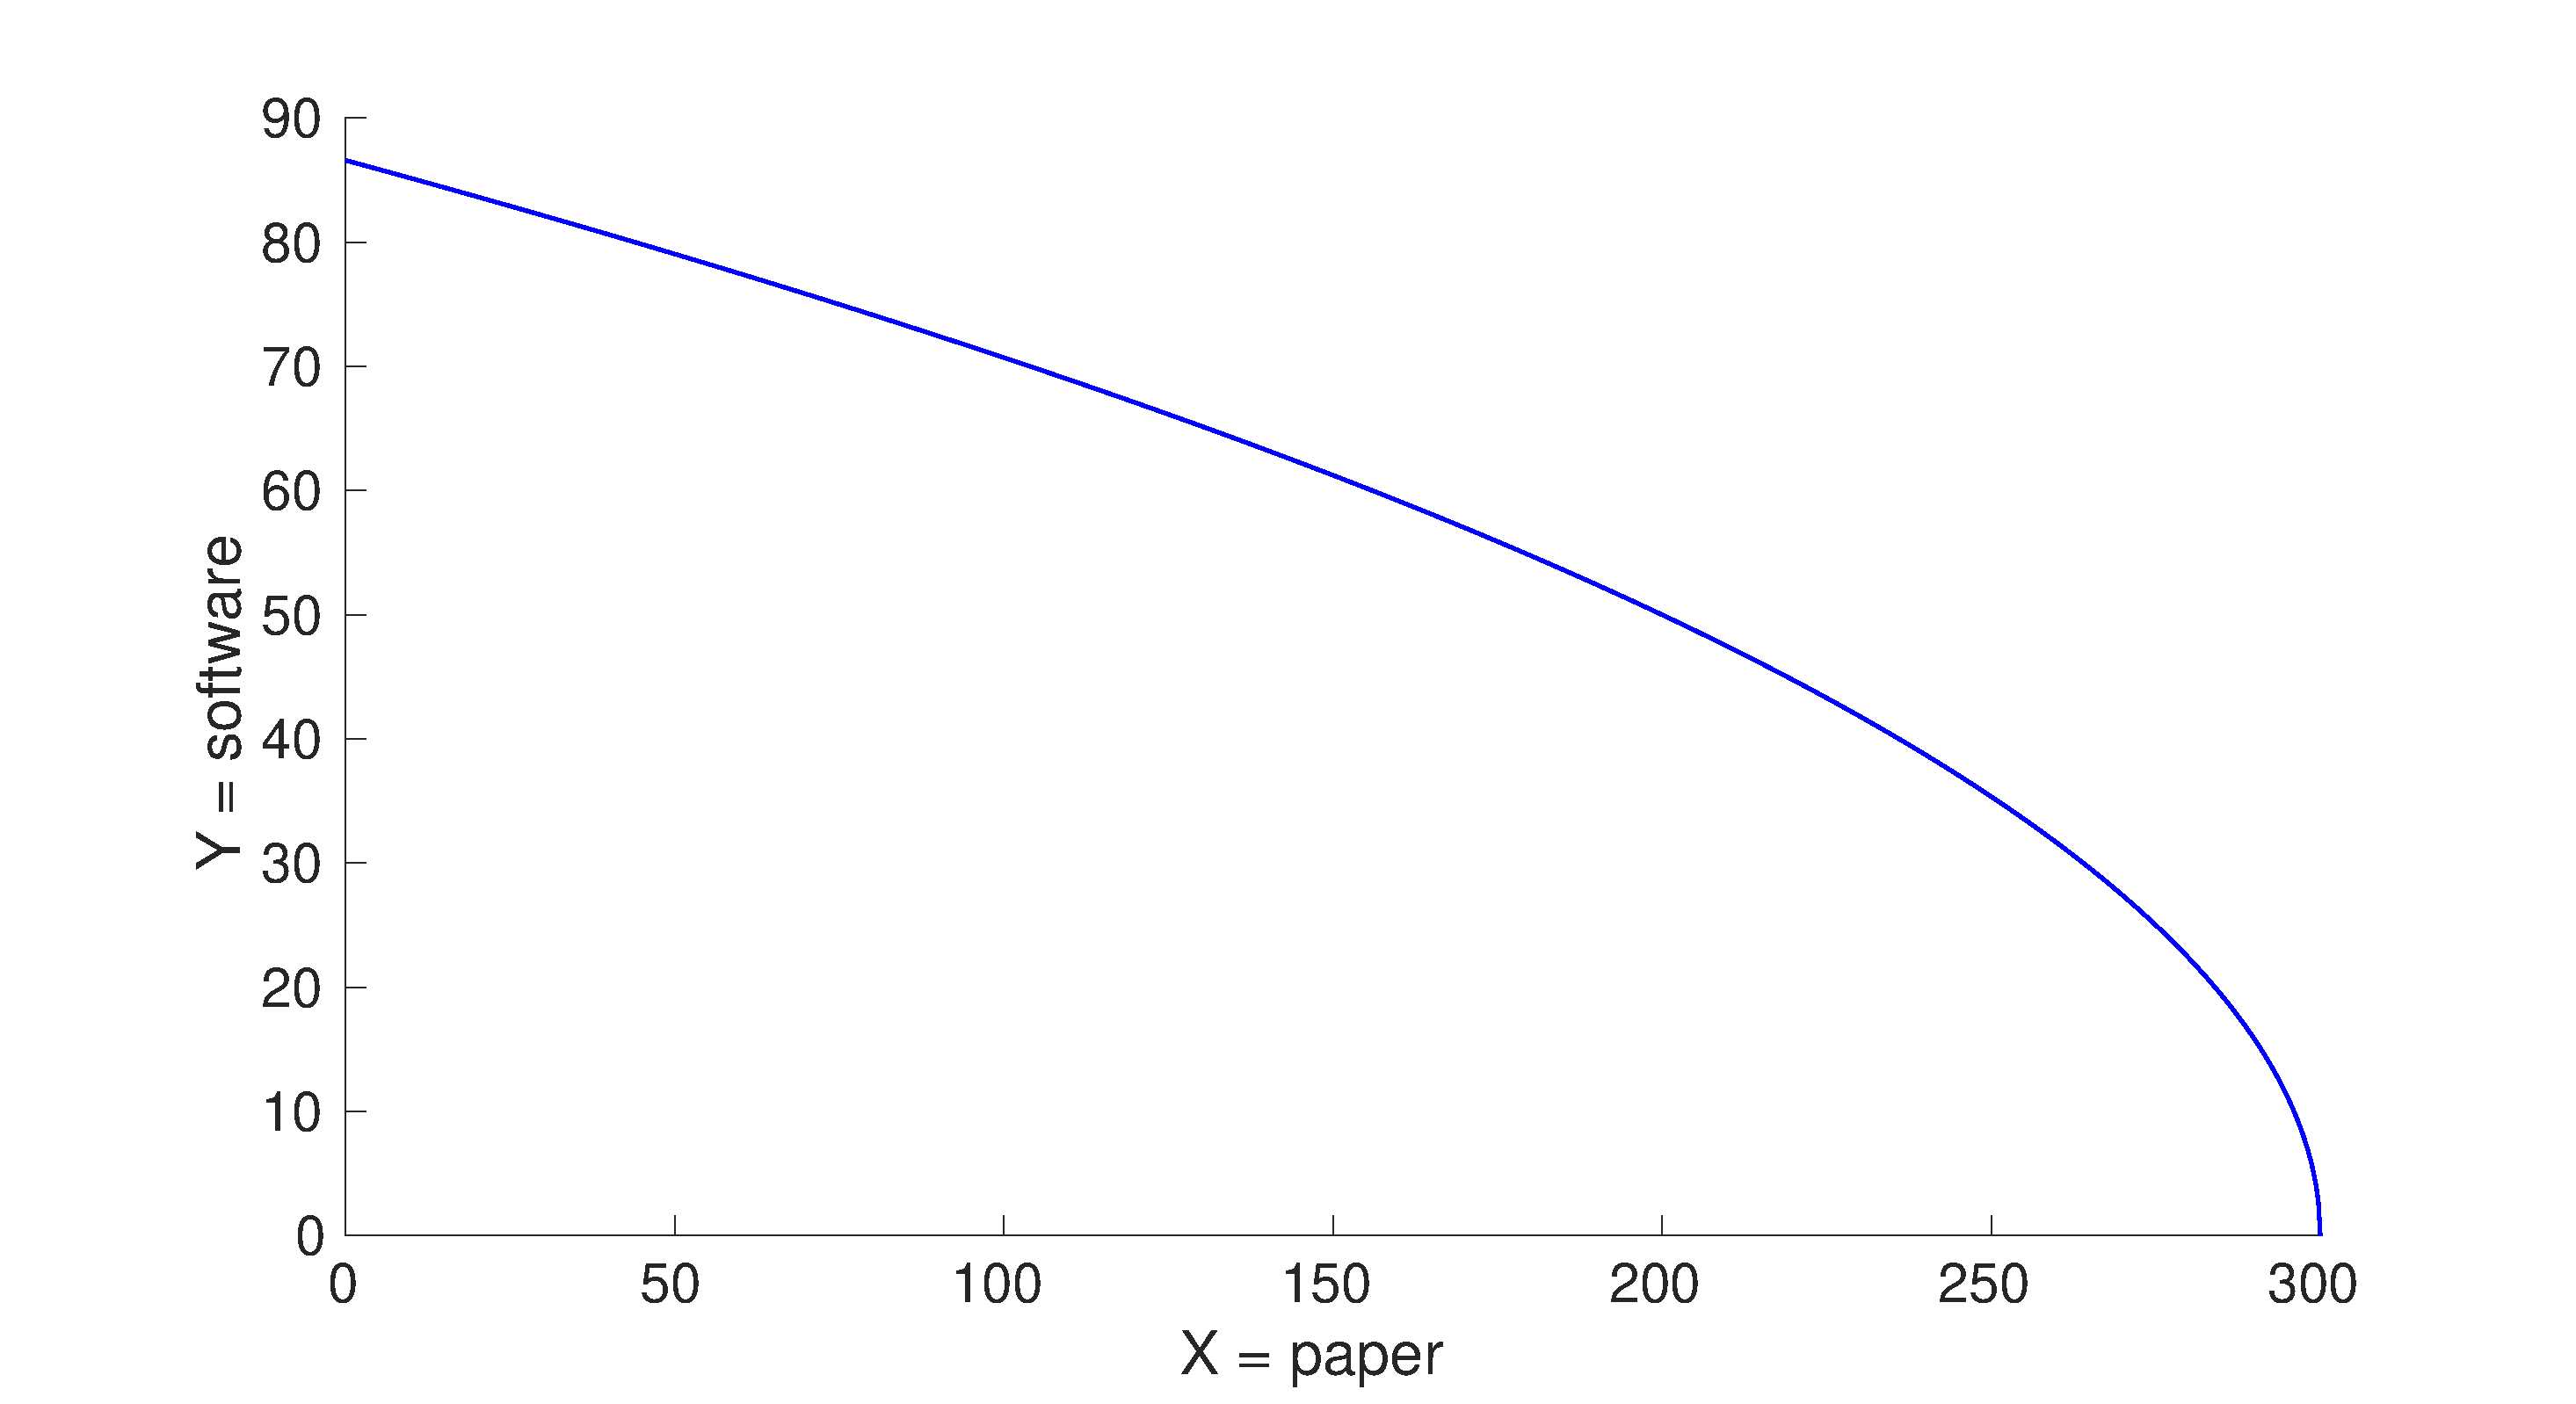
\includegraphics[width=12cm]{PPF.eps}\\
\caption{Finnish PPF for paper ($X$) and software ($Y$) production}\label{PPF}
\end{figure}

\subsection{Part 2}
MRS is given by
\begin{equation*}
\textup{MRS}_{XY}=\frac{\partial U/\partial X}{\partial U/\partial Y}=\frac{U/3X}{U/3Y}=\frac{Y}{X}
\end{equation*}

The PPF is
\begin{equation*}
\textup{PPF}(X,Y)=X+\frac{1}{25}Y^2-300=0
\end{equation*}

MRT is given by
\begin{equation*}
\textup{MRT}_{XY}=\frac{\partial\textup{PPF}/\partial X}{\partial\textup{PPF}/\partial Y}=\frac{1}{2Y/25}=\frac{25}{2Y}
\end{equation*}

\subsection{Part 3}
If Finland does not trade with other countries, its MRS must equal MRT. Also, the bundle must lie on the PPF curve.
\begin{align*}
&\frac{Y}{X}=\frac{25}{2Y}\\
&X+\frac{1}{25}Y^2=300
\end{align*}

The solution is
\begin{equation*}
(X^A,Y^A)=(200,50)
\end{equation*}
where the superscript $A$ stands for autarky. So Finland produces 200 units of paper ($X$) and 50 units of software ($Y$).

The equilibrium price ratio is
\begin{equation*}
\frac{P^F_Y}{P^F_X}=\textup{MRT}_{YX}=\frac{1}{\textup{MRT}_{XY}}=\frac{2Y^D}{25}=4
\end{equation*}

\subsection{Part 4}
Since $P^U_X=P^F_X=1$ and $P^U_Y>P^F_Y$, the US has comparative advantage over paper ($X$) and Finland has comparative advantage over software ($Y$). Therefore, if trade begins, Finland will export software and the US will export paper.

Since $P^U_X=P^F_X=1$, to result in no trade, the US software price must equal that of Finland: $P^U_Y=P^F_Y$.

\subsection{Part 5}
Let MRT equal the price ratio.
\begin{equation*}
MRT_{XY}=\frac{25}{2Y}=\frac{P_X^I}{P_Y^I}=\frac{1}{4.8}
\end{equation*}
which gives $Y^T=60$, where the superscript $T$ stands for trade. Consequently, $X^T=300-(Y^T)^2/25=156$. So Finland produces 156 units of paper ($X$) and 60 units of software ($Y$). The GDP is
\begin{equation*}
\textup{GDP}=P_X^IX^T+P_Y^IY^T=1\times 156+4.8\times 60=444
\end{equation*}

\subsection{Part 6}
We try to maximize $U(X,Y)=X^{1/3}y^{1/3}$ subject to the constraint that $P_X^IX+P_Y^IY\leqslant\textup{GDP}=444$. Introduce a Lagrange multiplier $\lambda$,
\begin{equation*}
L(X,Y,\lambda)=X^{1/3}Y^{1/3}-\lambda(X+4.8Y-444)
\end{equation*}

Taking partial derivatives with respect to $X,Y$ and $\lambda$ and setting them to zero,
\begin{align*}
&\frac{1}{3}X^{-2/3}Y^{1/3}=\lambda\\
&\frac{1}{3}X^{1/3}Y^{-2/3}=4.8\lambda\\
&X+4.8Y=444
\end{align*}

The solution is
\begin{equation*}
(X^*,Y^*)=(222,46.25)
\end{equation*}

Therefore, the excess demand of paper ($X$) is $\Delta X=X^*-X^T=222-156=66$, and the excess demand of software ($Y$) is $\Delta Y=Y^*-Y^T=46.25-60=-13.75$. This means Finland will import 66 units of paper and export 13.75 units of software.

In the autarky case, Finnish utility is
\begin{equation*}
U^A=(X^A)^{1/3}(Y^A)^{1/3}=(200\times 50)^{1/3}\approx21.54
\end{equation*}

In the trading case, Finnish utility is
\begin{equation*}
U^T=(X^*)^{1/3}(Y^*)^{1/3}=(222\times 46.25)^{1/3}\approx21.73
\end{equation*}

Since $U^T>U^A$, a representative Finnish consumer is better off when Finland opens to trade.

\subsection{Part 7}
Since Finland produces more software and less paper when it opens to trade, some workers in the paper industry have to move to the software industry. They suffer from a loss. Therefore, workers of the paper industry will oppose to international trade with the US.

\subsection{Part 8}
They fail to consider the fact that absolute productivity of labor / absolute market price does not affect the decision of opening to trade. It is the comparative advantage that matters. Since the US paper industry is twice more productive than that in Finland, but its software industry is only 1.6 times more productive than that in Finland, we conclude that the US comparative advantage lies in paper industry. Then the US should open trade with Finland by exporting paper and importing software.

\section{Externalities}
\subsection{Part 1}
The total revenue of company A is
\begin{equation*}
\textup{TR}_A=N(20N^{-1/2}-C)=20N^{1/2}-N
\end{equation*}

To maximize $\textup{TR}_A$, set its partial derivative with respect to $N$ to zero.
\begin{equation*}
\frac{\partial\textup{TR}_A}{\partial N}=10N^{-1/2}-1=0
\end{equation*}

The solution is $N=100$. So company A should take 100 tourists per day.

\subsection{Part 2}

\end{document}
